\documentclass[12pt]{article}
\usepackage{helvet}
\renewcommand{\familydefault}{\sfdefault}
\usepackage[letterpaper, top=1.2in, bottom=1.2in, left=1.2in, right=1.2in, heightrounded]{geometry}
\linespread {1.15}
\usepackage{graphicx}
\graphicspath{ {./assets/img} }
\author {Alexis Aoun}
\begin{document}
\begin {sloppypar}
\title {Stage Atos}
\date {}
\maketitle
\newpage

\def\contentsname{Sommaires}
\tableofcontents
\newpage

\renewcommand{\listfigurename}{Table des matières des illustrations}
\listoffigures
\newpage

\section*{Résumé et mots clés}
\addcontentsline{toc}{section}{Résumé et mots clés}
\paragraph{}
Dans le cadre de mon stage de M1 j'ai travaillé en tant que développeur d'application 
web pendant 4 mois au sein d'Atos, une multinationale dans le domaine du numérique. 
J'ai eu l'occasion de contribuer à trois projets : MPP Dashboard qui est une application 
devant rappeler automatiquement par mail les employés d'accomplir des demandes administratives, 
Tickeratops qui est un outil de gestion de tickets et d'automatisation de tâches de devOps, et enfin 
le projet client UGAP où je suis intervenu dans la rénovation de l'interface graphique d'un site web. 
J'ai acquéris un large pannel de compétences techniques dans le domaine des applications web à la fois 
pour le développement d'interface graphique mais aussi dans la programmation de serveur web gérant les données.
Je me suis aussi et surtout familiarisé avec les méthodes Agiles pour la gestion des projets et des équipes.
\paragraph{}
Mots clés : Digitalisation, application web, frontend, backend, Javascript
\newpage

\section*{Abstract and keywords}
\addcontentsline{toc}{section}{Abstract and keywords}
\paragraph{}
As part of my fourth year in IMT Nord Europe I did an intership as a web developer for 4 months 
in Atos, a multinational company in the digital field. I had the occasion of contributing to 3 projects : 
MPP Dashboard which is an application that is designed to warn employees by email automatically to accomplish certain 
administrative duties, Tickeratops which is a ticket management tool and an automatisation utility for devOps tasks and 
finally a client project named UGAP where I was assigned in the frontend redesign team. I gained a large set of technical 
skills ranging from frontend building to backend server development. I also familiarized myself 
with the Scrum framework used for project and team management.
\paragraph{}
Keywords : Digitalizaton, web application, frontend, backend, Javascript
\newpage

% gantt 
\section*{Planning global de mon stage}
\addcontentsline{toc}{section}{Planning global de mon stage}
\begin{figure}[h]
  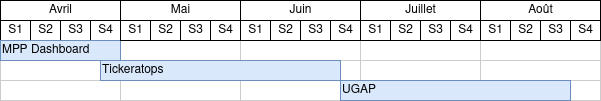
\includegraphics[width=\textwidth] {gantt.png}
  \caption {Diagramme de Gantt de mon stage}
\end{figure}
\newpage

% introduction 
\section{Introduction}
\paragraph{}
Dans le cadre de mon année de M1, j'ai effectué un stage de 4 mois au sein de l'entreprise 
Atos, sur leur site lillois. J'ai eu l'occasion de travailler en tant que développeur d'application 
web sur trois projets, deux internes et un pour un client externe. Dans le rapport qui suit je vais exposer le contexte 
de réalisation du stage, suivi par une présentation des missions entreprises et les résultats obtenus pour chaque projet,
et enfin je ferais un bilan des compétences acquises ainsi que de l'état de mon projet de parcours professionnel. 

% 1 - Presentation
\section{Contexte de réalisation du stage}
\subsection{Présentation d'Atos}
\paragraph{}
Atos est une Entreprise de Services du Numérique (ESN) française née de la fusion de 
deux entreprises (Axime et Sligos) en 1997. C’est une entreprise leader européen du cloud, 
et leader international du numérique sécurisé et décarboné. Présent dans 
le monde entier, Atos se pose comme étant l’une des dix plus grandes ESN au niveau mondial.

\paragraph{}
\begin{figure}[h]
  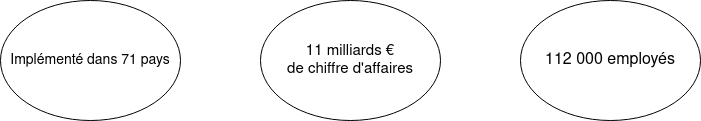
\includegraphics[width=\textwidth] {chiffres-cles.png}
  \caption {Chiffres clés d'Atos}
\end{figure}

\subsection{Les partenaires}
\paragraph{}
La notoriété et l'ancienneté d'Atos font que l'entreprise possède un nombre conséquent 
de partenaires. Voici une liste des plus importants : 
\paragraph{}
Amazon Web Service, Dell Technologies, Google Cloud, Microsoft, Siemens, VW Ware, Cisco, IBM, Oracle,
Hitachi, Red Hat, ServiceNow, Salesforce.

\subsection{L'organisation}
\subsubsection{Organisation générale}
\paragraph{}
Atos étant une grande multinationale elle possède un système organisationnel développé 
autour de la position géographique de ces différentes Business Unit ou Unité commerciale
en français. 

\begin{figure}[h]
  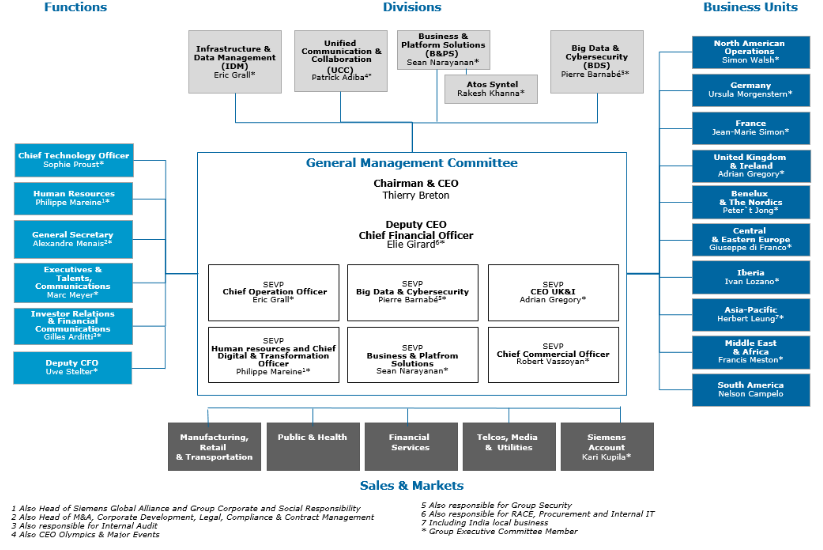
\includegraphics[width=\textwidth] {orga_atos.png}
  \caption {Organisation d'Atos - 2019 }
\end{figure}

\subsubsection{L'entité Cloud Apps and Data}
\paragraph{}
Mon stage s'est déroulé dans l'entité Cloud Apps and Data, ou CAD, gouvernée par 
l'unité commerciale France. Celle-ci est constitué d'une soixantaine de développeurs et de devOps$^{1}$ qui produisent 
des solutions digitales dans le cadre de projets internes et projets clients externes.
Voici une courte liste non-exhaustive des clients prises en charge par le CAD : Auchan, Pierre-Fabre, Sncf, UGAP, Kiabi,
 la Ratp et bien d'autres.

\subsection{La politique d'Atos}
\paragraph{}
Étant une entreprise pionière dans la digitalisation, Atos se doit d'être à la pointe
des dernières technologies. C'est pour cette raison qu'elle se dote d'une politique 
de R\&D aggréssive notamment dans les domaines du Cloud, de l'intelligence artificielle 
et du traitement des données.
\paragraph{}
Atos fournit aussi une attention particulière à son empreinte carbonne et à respecter ses reponsabilités environnementales
en s'engageant à réduire de 50\% ses émissions entre 2019 et 2025 et de 90\% au plus tard en 2039 
% 2 - missions
% MPP
\newpage
\section {Objectifs et réalisation de mes missions}
\subsection {MPP Dashboard}
\subsubsection {Le contexte} \paragraph {}
Atos a une plateforme en ligne, My Atos, sur laquelle tous les employés doivent 
renseigner leurs informations personnelles ainsi que leurs parcours professionnel et 
académique. Le problème de cette procédure, qui est en théorie obligatoire, est qu' 
une partie importante des salariés ne remplissent pas ces informations, et la plupart 
du temps cela est dû à un simple oubli. Pour y remédier, le service RH et la direction 
général d'Atos décidèrent de lancer un projet interne qui permetterait de relancer 
les employés automatiquement à partir d'un fichier excel contenant les informations 
de tous les collaborateurs, fournit par le service RH. Ce projet fut baptisé MPP Dashboard.

\paragraph {} 
Le projet est une application web dont le fonctionnement repose sur trois processus
principaux : 
\begin {enumerate}
  \item 
    Le traitement de l'excel : Le service RH fournit un fichier excel sous format XSLX 
    (Le format par défaut des fichiers excels microsoft). Celui-ci doit être traité de 
    manière à ce que les informations qu'il contient puissent être manipuler 
    programmatiquement.
  \item 
    Le filtrage : Une fois les donnés des collaborateurs dans notre application, on
    sauvegarde dans une base de données uniquement ceux dont le taux de renseignement 
    d'informations et en-dessous d'un seuil défini par les administrateurs de 
    l'application. Le taux par défaut est de 90\%. 
  \item 
    L'envoie de mail : L'application enverra des mails à tous les salariés présent 
    dans la base de données après la phase de filtrage. Un chiffre correspondant au nombre
    de mails envoyés aux collaborateurs est associé à chacun d'entre eux. Au bout du 
    5ème mail l'employé n'ayant pas renseigner les informations nécéssaires est signalé 
    automatiquement au service RH.
\end{enumerate}
\newpage
\begin{figure}
  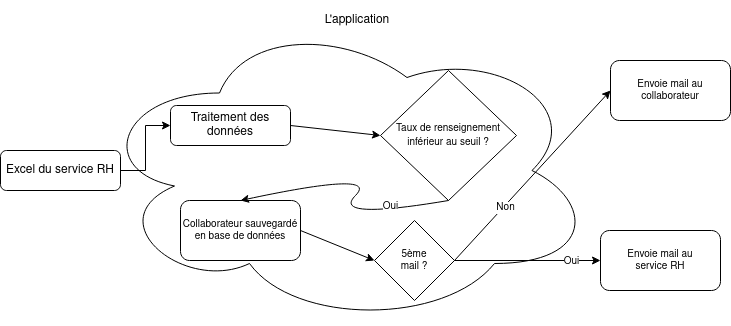
\includegraphics[width=\textwidth] {mpp-diagram.png}
  \caption {Diagramme du fonctionnement de MPP Dashboard}
\end{figure}
\paragraph {}
Les technologies utilisés pour la réalisation du projet sont : 
\begin {itemize}
\item   
  Pour la base de données : PostgreSQL$^{2}$ 
\item 
  Pour le serveur backend$^{3}$ : ExpressJS$^{4}$
\item 
  Pour l'interface grahique : ReactJS$^{4}$
\end {itemize}

\subsubsection{La problèmatique}
\paragraph {}
Lorsque je suis arrivé sur le projet, celui-ci a déjà été développé mais avait un 
problème avec l'un des processus, celui d'extraction de l'excel. En effet la librairie$^{5}$
utilisée pour remplir cette tâche, du nom d'Excellente, a été développée en interne par des 
employés d'Atos et comporte certains inconvénients : 
\begin{itemize}
  \item 
    Il comporte plusieurs bugs$^{6}$. Cela est notamment dû au fait que cette librairie 
    n'est pas connue du grand publique et ne reçoit donc pas un grand nombre de tests et 
    de contributions 
  \item 
    La librairie devient exponentiellement lente avec la grandeur du fichier excel. Hors
    celui qu'on a à extraire fait plus de 40 000 lignes
\end{itemize}
Ma tâche est donc de trouver une solution qui puisse répondre à la fois aux problèmes
de vitesse et de fiabilité.
\newpage
\subsubsection{Les solutions possibles}
\paragraph {}
Afin d'accomplir ma mission j'ai étudié plusieurs possibilités : 
\begin{itemize}
  \item 
    Garder la librairie Excellente et essayer de gommer ces défauts en modifiant
    son implémentation, voir même la librairie en elle-même. 
    Le risque est que cela prenne trop de temps ou même que cela n'aboutisse tous 
    simplement pas. Du fait de l'utilisation limitée d'Excellente et du manque de documentation 
    techique, corriger la librairie pourrait prendre des mois alors que la direction d'Atos 
    attendait des résultats dans les semaines suivant mon arrivé.
  \item 
    Utiliser un script Python$^{7}$. Lors de mes différents cours en data au sein de l'IMT Nord 
    Europe, l'une des compétences que j'ai acquis est le traitement de données par le biais 
    de script Python en utilisant des librairies tels que Panda$^{8}$. Les performances 
    seraient des ordres de grandeurs meilleurs que celle de n'importe quelle autre solution 
    implémentée en Javascript$^{9}$, et l'écriture du script peut se faire en une journée. 
    La difficulté est l'implémentation du pont entre le serveur ExpressJS et le script Python. 
    Celui-ci doit être exécuter au bon moment par le serveur, et ce dernier doit pouvoir 
    récupérer le résultat final. Il y avait aussi la problématique des dépendances$^{10}$ spécifique
    à Python dont a besoin un tel script qui rajouterait une couche de compléxité au projet ExpressJS, au 
    développement mais surtout à la maintenance.
  \item 
    Utiliser une autre librairie Javascript, ExcelJS. ExcelJS est sans aucun doute 
    la librairie Javascript la plus utilisée pour le traitement d'excel. Un avantage très important 
    d'une librairie aussi connue est sa documentation riche qui m'a permis de faire des premiers 
    tests rapidements. De ces expérimentations j'en avais conclu que la fiabilité était 
    satisfasante et que la vitesse était tout à fait convenable pour notre application, même si 
    plus lente que le script Python. Cette solution fut donc retenu.
\end{itemize}
\newpage
\subsubsection{La réalisation de la mission}
\paragraph{}
La mise en œuvre de la solution fut assez simple dans son ensemble en grande partie 
grâce à l'excellente documentation d'ExcelJS. La seule difficulté rencontrée a été la gestion 
des erreurs dans l'excel. En effet celui-ci comporte des formules qui dans certains cas retournent
des erreurs. Mon implémentation a donc dû prendre en compte ces cas de figures là. Après cela j'ai pu 
procéder à une série de tests sur mon ordinateur personnel, le traitement de l'excel comportant 40 000
lignes a duré dans les alentours des 1 minutes et 45 secondes. Il était temps de déployer ma solution 
en production.
\subsubsection{Résultats et bilan}
\paragraph{}
Après quelques ajustements mon algorithme de traitement obtenait les résultats escomptés.
Le temps d'exécution de moins de 2 minutes jugés satisfasant. 
\linebreak 
Avec plus de temps une implémentation du script Python aurait été possible, permettant de réduire encore
plus le temps de traitement. Néanmoins je pense avoir pu obtenir le meilleur résultat possible 
compte tenu de la contrainte temporelle.
\paragraph{}
Cette première mission fut l'opportunité pour moi de prouver à la fois mes compétences techniques
mais surtout mes capacités à prendre des initiatives et à les mettre en œuvre.

%Tickeratops
\newpage
\subsection{Tickeratops}
\subsubsection{Le contexte}
\paragraph{}
Comme mentionné dans la partie décrivant le contexte de réalisation de mon stage, j'ai évolué 
dans l'entité Cloud Apps \& Data, ou CAD. Celle-ci est composée principalement de deux corps 
de métier, les développeurs et les devOps qui travaillent ensemble afin de concevoir 
et déployer les solutions efficacement.
\paragraph{}
Cependant un problème récurrent apparait au sein de l'entité : la communication entre ces deux 
groupes. En théorie un canal de communication sur la plateforme Teams est dédié à l'échange 
entre développeur et devOps, mais le manque de formalisme et la forte pression que peuvent 
subir les devOps engendre un temps d'attente prolongé pour le traitement des demandes des développeurs
qui en conséquence décident souvent de court-circuiter Teams et de communiquer directement
avec les devOps soit en personnne soit par message privé. Cela à pour effet d'aggraver les problèmes
d'organisations et de suivi des demandes. 
\paragraph{}
Il y a aussi un second axe d'amélioration qui est l'optimisation du temps de travail des devOps. 
Un certains nombres de leurs tâches s'avèrerent être répétitives, tel que le redémarage, la suprresion,
ou le déploiement de serveurs. 
\paragraph{}
Afin de répondre à ces deux problématiques les équipes du CAD ont décidé de développer une application web,
Tickeratops, qui aura un système de tickets pour les demandes des développeurs, lesquels pourront être
traités et suivis par les devOps avec plusieurs status (à faire, en cours de traitement, bloqué, terminé)
et qui seront affichés sous forme de kanban. L'autre fonctionnalité principale qui la distingue des 
nombreuses solutions de gestions de projets existantes est l'intégration direct d'exécution de script dans
l'application. Prenons l'exemple d'un développeur qui a besoin qu'un serveur de pré-production soit redémarrer : 
il créera un ticket décrivant son besoin et le devOps, qui aura prédifini cette action avec un script, n'aura qu'a 
appuyé sur un boutton pour relancer le serveur. Une fois le redémarrage accompli le ticket sera catégorisé 
comme étant accompli. La demande du développeur est suivi de bout en bout et le devOps gagne du temps 
grâce à l'automatisation intégrée dans l'application.

\newpage
\paragraph{}
Les techonologies utilisées pour ce projet sont : 
\begin{itemize}
  \item 
    Pour la base de données : MongoDB$^{11}$
  \item 
    Pour le serveur backend : NestJS$^{12}$ et GraphQL$^{13}$
  \item 
    Pour l'interface graphique : NextJS$^{14}$ 
\end{itemize}

\paragraph{}
Dans le cadre de ce projet j'ai eu à accomplir plusieurs tâches, au niveau du serveur et au niveau de 
l'interface graphique. Je vais me concentrer sur une seule mission, que je juge avoir été la plus 
intéressante. Lorsqu'un développeur crée un ticket il a le choix de rajouter une description afin 
d'expliquer plus en détail sa demande. Dans cette description on souhaite également pouvoir insérer 
des images afin d'illustrer nos propos, qui pourrait être par exemple une capture d'écran. La consigne 
qui m'a été donnée était de pouvoir stocker ces photos nos pas sur le même serveur où foncitonne 
le backend de l'application mais sur un serveur tiers détenu par l'un des partenaire d'Atos, Google, 
avec leur service de Bucket GCP$^{15}$

\subsubsection{La problématique}
\paragraph{}
Cette tâche requiert une bonne connaissance de l'environnement backend or je n'avais pas utilisé 
NestJS par le passé. Je n'ai également jamais utilisé la plateforme GCP de google, qui d'ailleurs 
devait être configurer sur mesure pour notre projet. Je devais donc passer par les devOps,
leur transmettre les besoins de l'application afin qu'ils mettent en place l'instance de Bucket GCP.

\subsubsection{La réalisation de la mission}
\paragraph{}
Dans un premier temps je pris le soin de m'autoformer et d'acquérir les compétences nécessaires 
à l'accomplissemnt de la tâche. Une fois assez familier avec NestJS je me suis penché sur l'excelllente
documentation de l'API de Google pour la plateforme GCP afin de pouvoir implémenter correctement 
la solution à l'application. Ensuite j'ai communiqué avec les devOps, pour la première fois depuis 
le début de mon stage, pour la mise en place de la plateforme GCP de production. J'ai pu alors vivre 
par moi-même la raison de l'existence du projet sur lequel je travail. 

\subsubsection{Résultats et bilan}
\paragraph{}
Après quelques ajustements et correctifs, la fonctionnalité produisait le résultat attendu. On 
pouvait sauvegarder, supprimer et afficher des images de notre Bucket GCP à partir de l'
application web. 
\paragraph{}
A travers cette mission j'ai pu faire preuve d'adaptation en m'autoformant aux technologies 
requises. Mais là n'est pas la leçon la plus importante. Contrairement au projet MPP où j'étais 
seul, j'ai travaillé au sein d'une équipe qui suivait les principes des méthodes agiles ou SCRUM,
une première pour moi. J'ai donc appris les fondamentaux avec les sprints et les users story. 
J'ai également pu participé aux sprint review, sprint planning, retro, daily etc. Des connaissances 
basiques d'organisations d'équipes que je ne connaissais qu'en théorie.

% UGAP
\newpage
\subsection{UGAP}
\subsubsection{Le contexte}
\paragraph{}
Pour ma 3ème mission j'ai eu la chance de travailler sur un projet client externe. Une occurence 
rare chez Atos qui préviligie les projets internes pour les stagiares et alternants.
\begin{quote}
  "L’UGAP est un établissement public à caractère industriel et commercial français créé en 
  1985 et placé sous la double tutelle du ministre chargé du Budget et du ministre chargé de 
  l'Éducation nationale. Elle est une centrale d'achat publique généraliste et constitue, 
  en raison d'un mode opératoire quasi-exclusif en achat pour revente, un acteur spécifique de 
  l’achat public, dont le rôle et les modalités d’intervention sont définis par le code de 
  la commande publique (qui est entré en vigueur en avril 2019) relative aux marchés publics5. 
  Son activité globale concerne plus de cinq milliards d'euros hors taxes, 
  répartis en 4,67 milliards d'euros d'activité de grossiste (achat pour revente) et 520 millions d'euros 
  d'achats réalisés en direct par les entités publiques sur les marchés de gaz et d'électricité passés par 
  l'UGAP pour leur compte en tant qu'intermédiaire." \linebreak 
  https://fr.wikipedia.org/wiki/Union\_des\_groupements\_d'achats\_publics 
\end{quote}
Pour résumer en une phrase, la raison d'être d'Ugap est la vente de biens aux établissements publics.
\paragraph{}
Aujourd'hui la majorité des ventes se font à travers leur site internet. Celui-ci dattant de plus d'une décennie 
requiert d'être remis à niveau, à la fois visuellement et dans la gestion du backend. 
\newpage
\begin{figure}
  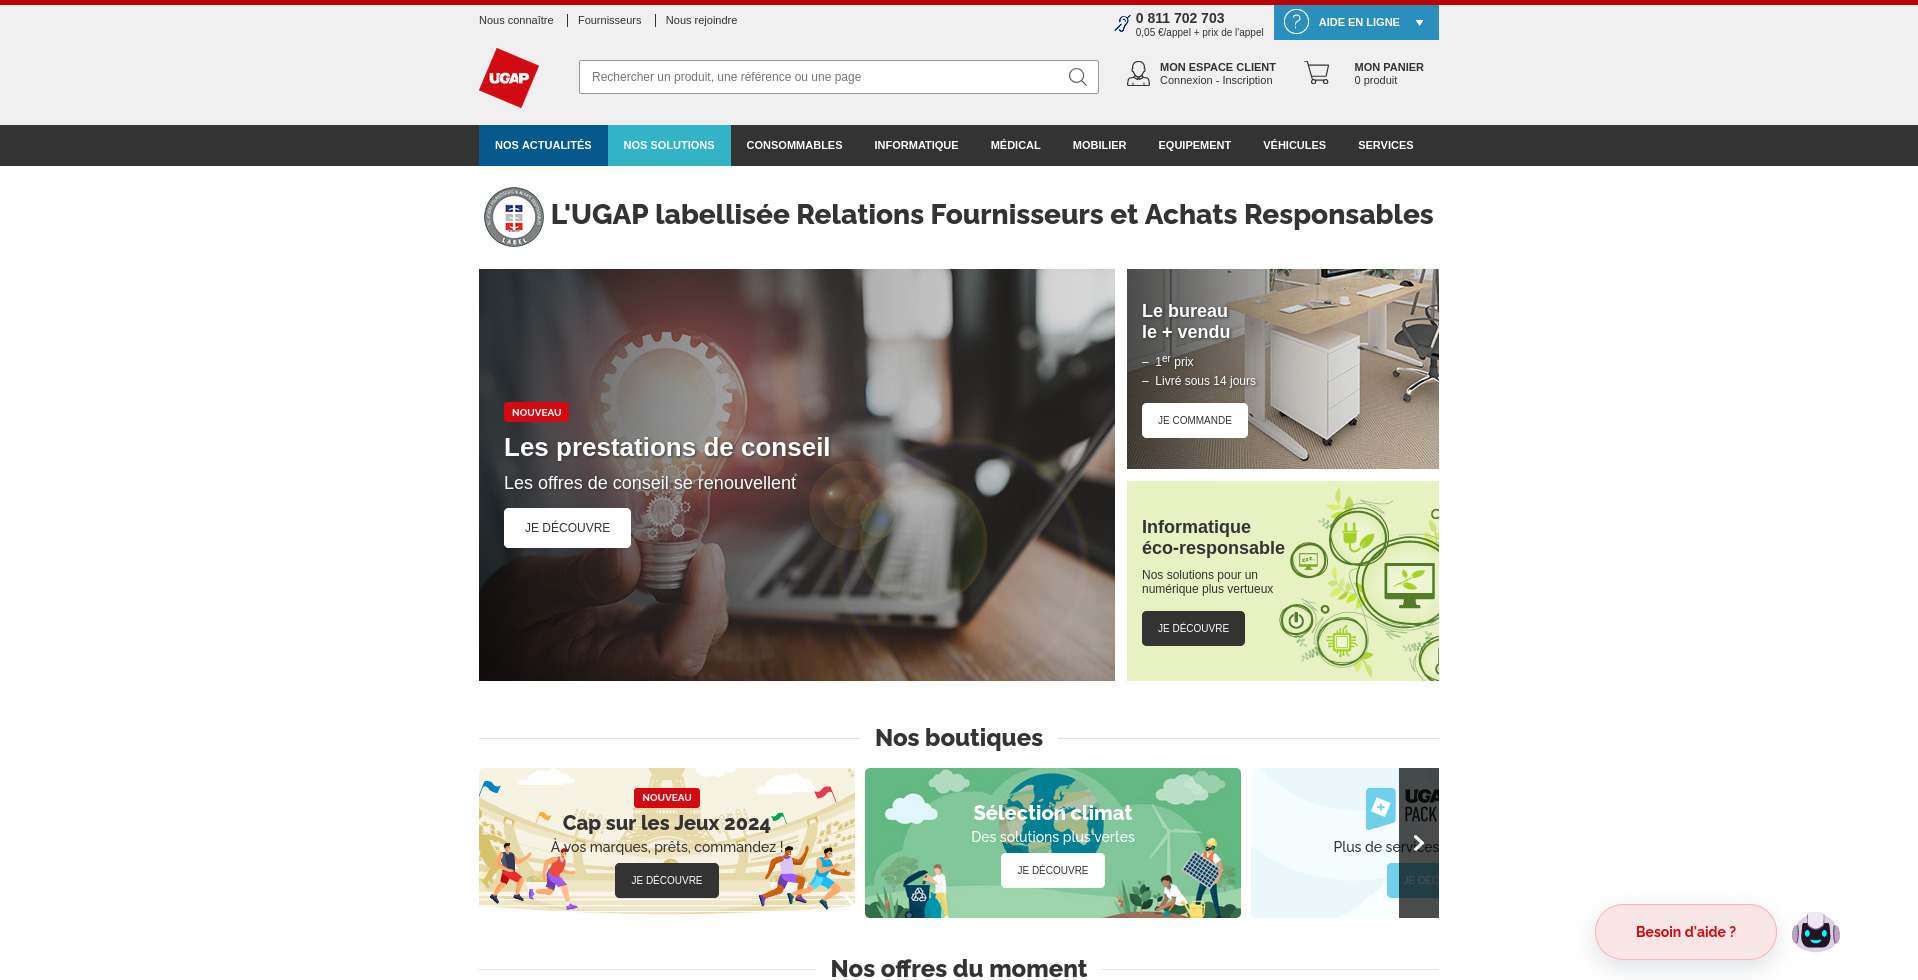
\includegraphics[width=\textwidth] {sc_ugap.png}
  \caption {Site actuel de l'Ugap}
\end{figure}
\paragraph{}
C'est dans ce contexte qu'intervient Atos en tant que préstataire extérieur avec pour mission de 
rénover le site. J'ai fait parti de l'équipe chargée de la refonte graphique. 
\paragraph{}
Je n'avais par le passé jamais participé à un projet d'une tel envergure, l'architecure et les outils 
techniques employés reflètent parfaitement bien la compléxité de l'application. L'interface graphique 
est composé de plusieurs microfrontend. Pour comprendre ce qu'est un microfrontend on peut faire 
l'analogie avec les micro-services utilisés communement dans les serveurs backend. La raison d'être 
des microservices est qu'au lieu d'avoir un gros serveur monolithique on ai plusieurs petites applications 
regroupés sous un même domaine$^{16}$. Cela permet de conteneuriser les fonctionnalités. Par exemple 
un supermarché peut décider d'avoir un microservice pour la gestion des produits, un autre pour la 
gestion des employés, un autre pour la gestion de l'inventaire etc. Un microfrontend se base sur le même 
principe à la différence qu'ici on ne conteneurise pas des fonctionnalités backend mais des interfaces 
graphiques.
\newpage
Le site d'Ugap est composé de trois grandes sections : 
\begin{itemize}
  \item 
    Section produit, pour l'achat de biens
  \item 
    Section offre, présentant les réductions et soldes du moment
  \item 
    Section magazine, contenant des articles sur l'actualité du service publique
\end{itemize}
\begin{figure}[h]
  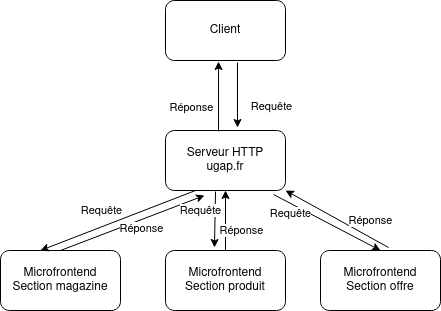
\includegraphics[width=\textwidth] {archi_ugap.png}
  \caption {Diagramme de l'architecture frontend du nouveau site d'Ugap}
\end{figure}
L'interface de chacune de ces sections est un microfrontend indépendant. Les avantages d'une telle 
architecture sont : 
\begin{itemize}
  \item 
    Un site plus robuste au bug et autres problèmes : Si l'un des microfrontend vient à ne plus 
    fonctionner le reste du site n'en sera pas impacté
  \item 
    Une maintenance plus simple : Pour les même raisons que le premier point, si l'on veut 
    mettre à jour l'une des sections on peut le faire sans avoir à désactiver l'ensemble du site 
  \item 
    Un développement en équipe facilité : L'indépendance inter microfrontend fait que les développeurs 
    des différentes sections n'apporteront pas de modifications qui peuvent rentrer en conflit
\end{itemize}
L'interface en elle-même est developpée avec NuxtJs$^{17}$ et VueJS$^{18}$. L'ensemble des tâches 
que j'ai effectué pour le projet Ugap s'est concentré sur la section produit, plus précisement 
la page produit. Cette page comporte la description du produit sélectionné et offre la possibilité 
de l'ajouter au panier pour l'acheter.
\begin{figure}[h]
  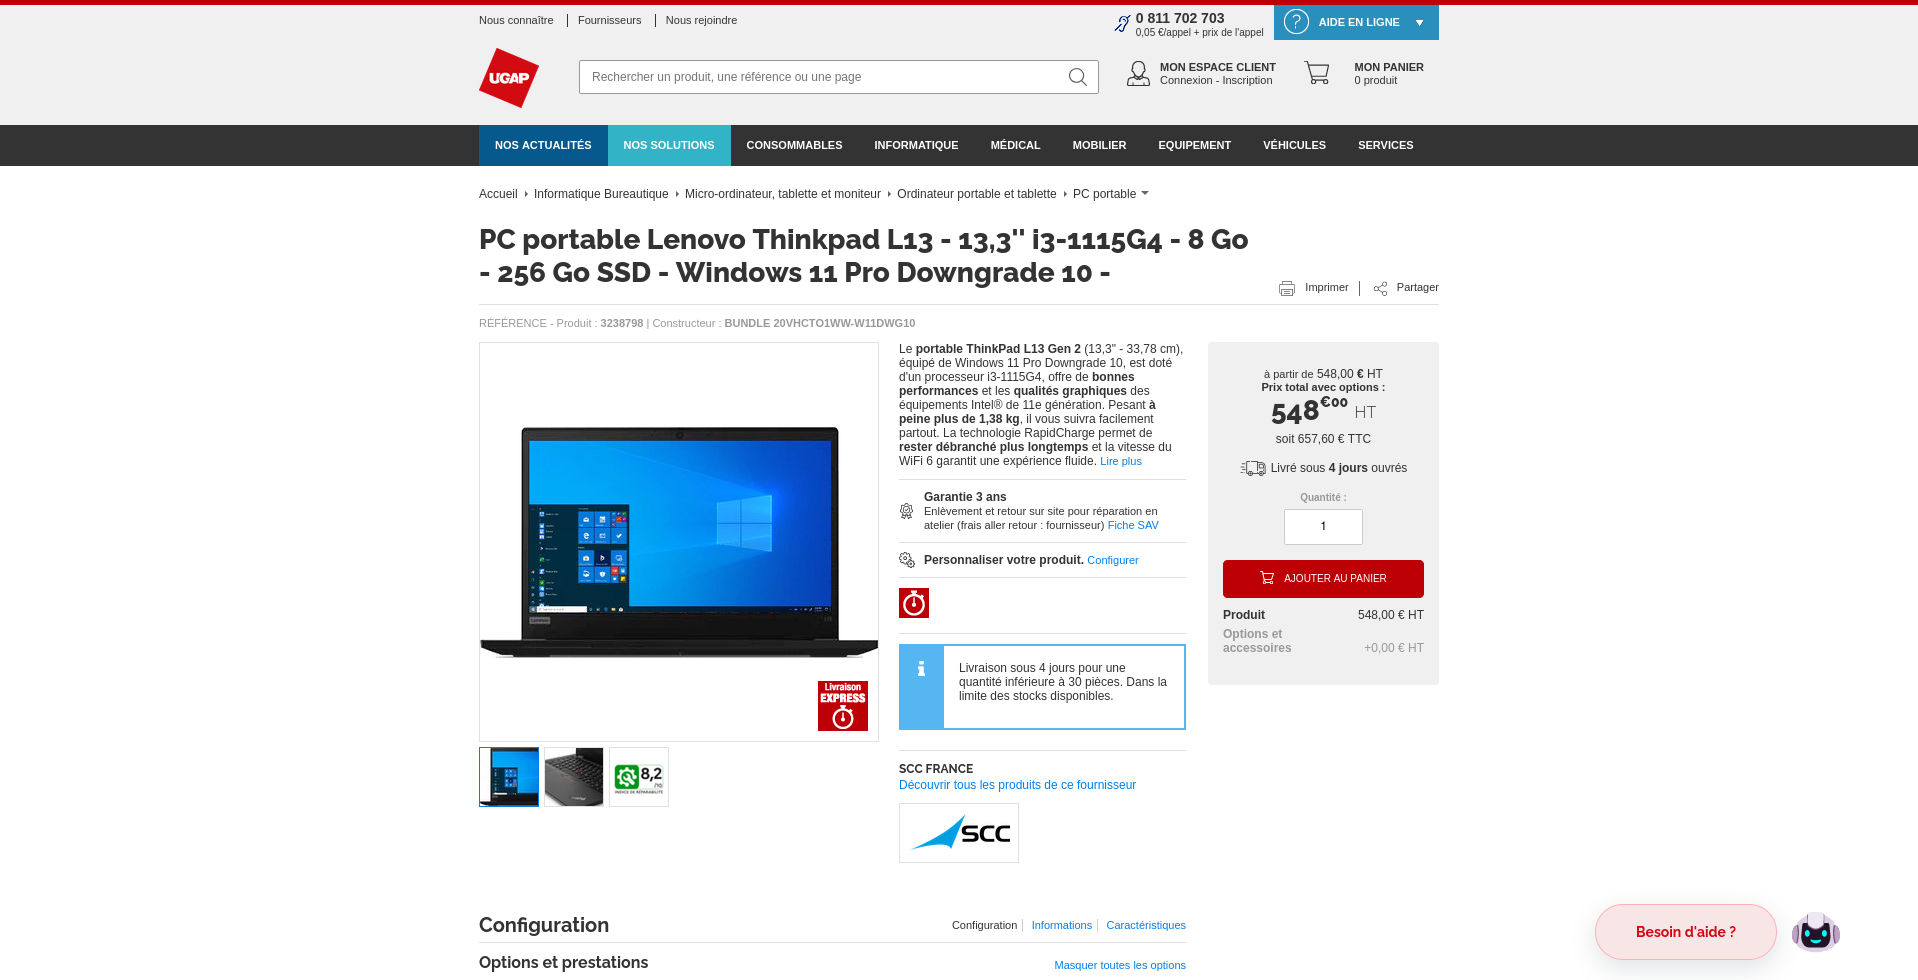
\includegraphics[width=\textwidth] {sc_product-page.png}
  \caption {Capture d'écran de la page produit du site actuel d'Ugap}
\end{figure}
\newpage 
\subsubsection{La problématique}
\paragraph{}
Il est évident que de comprendre une architecture aussi complexe avec une base de code aussi grande 
est une épreuve en soit, surtout qu'après avoir était sur deux autres projets différents en moins de 3 mois
une certaine fatigue commençait à apparaitre. Autre problème qui était général à l'ensemble du projet
et dont je fis état assez rapidement fut le manque de communication entre l'équipe frontend et backend. 
Or celle-ci est indispensable pour que l'on puisse savoir comment l'API$^{19}$ d'Ugap fonctionne et
surtout être au courant des futures changements auquel on doit s'adapter au niveau de l'interface,
par exemple le format dans lequel l'ont recevait les données. A noter que l'équipe s'occupant du 
backend était constituée et dirigée en majorité par des employés d'Ugap et non d'Atos, ce qui ne 
facilite pas la communication.
\subsubsection{Réalisation de ma mission}
\paragraph{}
J'ai commencé par des tâches simples comme l'amélioration ou la modification de composants graphiques
pré-existants. En parallèle je m'étais autoformé aux technologies utilisés pour la gestion des microfrontend 
afin d'avoir une compréhension plus profonde du projet sur lequel je travail. Je suis ensuite passé à des missions 
plus complexes comme la création d'un tableau affichant les différentes variantes d'un produit, par exemple
un ordinateur avec plusieurs processeurs différents. Quant aux problèmes de communication entre équipes frontend 
et backend j'ai essayé d'être à l'initiative avec mes collègues en créant des cannaux de conversations Teams 
et en remontant le problème aux différentes réunions afin d'initier la discussion autour du sujet.

\subsubsection{Résultats et bilan}
\paragraph{}
Au final j'ai réussi à accomplir la totalité des tâches qui m'ont été assignées. Le débat autour de la communication 
qu'on a provoqué avait commencé à porter ses fruits vers la fin de mon stage, les échanges devenaient plus 
fréquents, fluides et spontannés. 
\paragraph{}
J'ai grandement bénéficié de ce projet, évidement d'un point de vue technique, mais surtout d'un point 
de vue humain. D'abord j'ai encore plus approfondit mes connaissances en méthode Agile, avec notamment
la notion de swimlane et de weekly, mais j'ai aussi gagné à travailler dans une équipe aussi grande avec 
tant de métiers différents : développeurs, testeurs, designeurs d'interface, scrum master etc. Ce qui contraste
avec Tickeratops où l'on était une équipe de 5 développeurs et d'un scrum master. Je dois aussi mentionner
le sentiment unique à ce projet de travailler sur un produit qui se retrouvera à la disposition de milliers,
voir de dixaine de milliers d'utilisateurs, contrairement aux deux précédentes applications dont l'utilisation
sera limitée aux employés d'Atos. Ce sentiment de devoir se surpasser, de ne pas avoir le droit à l'erreur 
et d'être perfectionniste. Aujourd'hui j'attend avec impatience la mise en production du nouveau site 
prévu pour fin janvier et de voir le projet auquel j'ai contribué disponible au grand public.

\newpage
\section{Réflexion sur le métier d'ingénieur et la suite de mon projet professionnel}
\subsection{La contribution des ingénieurs au sein d'Atos}
\paragraph{}
Les ingénieurs sont au cœur de l'entreprise, c'est eux qui produisent la majorité de la valeur 
ajoutée que propose Atos. Ils sont perçus comme étant la "main d'œvre" de l'établissement.
\paragraph{}
Atos étant une grande multinationale la communication inter-entité est très procédurale et 
administrative. Cela à plusieurs inconvénients : 
\begin{itemize}
  \item 
    La lenteur des procédures qui peut causer des retards dans la progression des projets. Par exemple lors de mon travail 
    sur MPP Dashboard je devais résoudre une anomalie dans le système d'authentification. L'application utilise 
    le SSO$^{19}$ d'Atos et je devais donc m'assurer que l'instance du SSO pour l'application sur laquelle je travail 
    est toujours valide. Pour cela je devais communiquer avec l'entité responsable du SSO qui est localisé en Pologne 
    en remplissant un formulaire et en ouvrant un ticket sur une plateforme dédiée. Il m'a fallu attendre presque 
    deux semaines pour que le problème soit résolue, problème qui s'est avéré être une simple erreur de configuration
  \item 
    Le manque de contact humain entre les entités. Pour illustrer mes propos, des employés qui travaillait depuis
    des années dans l'entreprise ne connaissaient peu voir aucune personne de l'open space d'en face. Les 
    seuls fois où j'ai eu la chance durant mes 4 mois de stages de renconter des personnes d'autres entités étaient
    tout simplement durant mes pauses au baby foot de la caféteria de l'entreprise, et non durant mes heures de travail
\end{itemize}
\newpage
\subsection{Réflexion sur la suite de ma carrière}
\paragraph{}
Durant ce stage je me suis exclusivement concentré sur du développement web à la fois frontend
et backend. J'ai appronfondit mes compétences techniques avec de multiples librairies tel que NextJs,
NestJS etc.. et de nouvelles manières de concevoir des applications, avec le système de microfrontend
par exemple. Mais à mon sens l'acquis le plus précieux reste celui d'avoir travailler dans des équipes
dont la gestion se basée sur les méthodes Agiles. Quelques soit le domaine ou l'entreprise dans lequel je travaillerais 
à l'avneir ces connaissances resteront d'une constante utilité.

\paragraph{}
Si je devais refléter mon appréciation personelle sur le travail que j'ai accompli, il est évident que j'ai préfèré
le travail sur les serveurs et les bases de données. La conception et mise en place d'interface n'est clairement pas ce 
que je souhaite faire à l'avenir. Cette préférence ne fait que conforter mon plan pour la suite de ma carrière 
de devenir data scientist. Avec maintenant un stage de L2 en data, et un stage L3 et M1 en web, mon objectif 
est d'obtenir un PFE dans mon métier de prédilection. Mes compétences en développement web étant un bonus
non-négligeable qui pourra très certainement m'ouvrir des opportunités à l'avenir.

\section{Conclusion}
\paragraph{}
Ces 4 mois passés chez Atos m'ont apporté un baggage que je vais conserver très certainement tout 
au long de ma carrière. Non pas par les compétences acquises mais par l'expérience de travailler 
dans une entreprise multinationale. En effet mes stages précédents se sont tous réalisés dans des PME. 
L'un de mes objectifs étant de travailler en tant que data scientist pour un géant du numérique, 
de pouvoir m'approprier la culture, l'ambiance et la vie en général d'une entité de cette envergure
est la pièce qui manquait à ma préparation personnelle pour me lancer dans la réalisation de mon plan de carrière. 

\newpage
\section{Glossaire}
\begin{enumerate}
  \item 
    DevOps : Le devops — ou DevOps (selon la graphie habituellement utilisée en langue anglaise) —
    est un mouvement en ingénierie informatique et une pratique technique visant à l'unification du développement logiciel (dev) et de l'administration des infrastructures informatiques (ops), notamment l'administration système. 
    - https://fr.wikipedia.org/wiki/Devops
  \item 
    PostgreSQL : PostgreSQL est un système de gestion de base de données relationnelle et objet (SGBDRO). C'est un outil libre disponible selon les termes d'une licence de type BSD. 
    - https://fr.wikipedia.org/wiki/PostgreSQL
  \item 
    Backend : Lorsqu'un client envoie une requête à un serveur pour récuperer ou envoyer des données se serveur est considéré un serveur backend
  \item 
    ExpressJS : Express.js est un framework pour construire des applications web basées sur Node.js4. C'est de fait le framework standard pour le développement de serveur en Node.js5. L'auteur original, TJ Holowaychuck, le décrit comme un serveur inspiré de Sinatra6 dans le sens qu'il est relativement minimaliste tout en permettant d'étendre ses fonctionnalités via des plugins. 
    - https://fr.wikipedia.org/wiki/Express.js
  \item 
    Librairie : En informatique, une bibliothèque logicielle est une collection de routines, qui peuvent être déjà compilées et prêtes à être utilisées par des programmes1,2.
    Les bibliothèques sont enregistrées dans des fichiers semblables, voire identiques aux fichiers de programmes3, sous la forme d'une collection de fichiers de code objet rassemblés2 accompagnée d'un index permettant de retrouver facilement chaque routine3. Le mot " librairie " est souvent utilisé à tort pour désigner une bibliothèque logicielle. Il s'agit d'un anglicisme fautif dû à un faux-ami (library). 
    - https://fr.wikipedia.org/wiki/Biblioth\%C3\%A8que\_logicielle
  \item 
    Un bug : En informatique un bug est un dysfonctionnement ou anomalie présent dans un programme. 
  \item 
    Python : Un langage de programmation souvent utilisé dans le domaine de la data. 
  \item 
    Panda : Librairie Python facilitant la manipulation et la conversion de données en plusieurs formats. 
  \item 
    Javascript : Langage informatique utilisé en développement web. 
  \item 
    Dépendance : Une dépendance logicielle est le fait d'avoir besoin d'un logiciel donné pour en utiliser un autre ou le fait que la valeur de X influe sur le comportement de Y. 
    - https://fr.wikipedia.org/wiki/D\%C3\%A9pendance
  \item 
    MongoDB : MongoDB (de l'anglais humongous qui peut être traduit par " énorme ") est un système de gestion de base de données orienté documents, répartissable sur un nombre quelconque d'ordinateurs et ne nécessitant pas de schéma prédéfini des données. Il est écrit en C++. Le serveur et les outils sont distribués sous licence SSPL, les pilotes sous licence Apache et la documentation sous licence Creative Commons2. Il fait partie de la mouvance NoSQL. 
    - https://fr.wikipedia.org/wiki/MongoDB
  \item 
    NestJS : NestJS est un framework permettant la création de serveur web.
  \item 
    GraphQL : GraphQL1 (pour Graph Query Language) est un langage de requêtes et un environnement d'exécution, créé par Facebook en 2012, avant d'être publié comme projet open-source en 20152. Inscrit dans le modèle Client-Serveur, il propose une alternative aux API REST
    - https://fr.wikipedia.org/wiki/GraphQL
  \item 
    NextJS : Next.js2 est un framework gratuit et open source s'appuyant sur la bibliothèque JavaScript React3 et sur la technologie Node.js. 
    - https://fr.wikipedia.org/wiki/Next.js
  \item 
    Google Cloud Platform (GCP) est une plateforme de cloud computing fournie par Google, proposant un hébergement sur la même infrastructure que celle que Google utilise en interne pour des produits tels que son moteur de recherche1. Cloud Platform fournit aux développeurs des produits permettant de construire une gamme de programmes allant de simples sites web à des applications complexes
    - https://fr.wikipedia.org/wiki/Google\_Cloud\_Platform
  \item 
    Domaine : Un nom de domaine (NDD en notation abrégée française ou DN pour Domain Name en anglais) est, dans le système de noms de domaine DNS, un identifiant de domaine internet. Un domaine est un ensemble d'ordinateurs reliés à Internet et possédant une caractéristique commune. 
    - https://fr.wikipedia.org/wiki/Nom\_de\_domaine
  \item 
    NuxtJS : Nuxt.js est un framework gratuit et open source basé notamment sur Vue.js et Node.js. Le framework est présenté comme un " meta-framework pour créer des applications universelles ". Le terme " universel " signifie que le code de l'application est initialement exécuté par le serveur et ensuite dans le navigateur client4,5. L'application construite peut ainsi être utilisée dans un navigateur comme une application web monopage mais elle peut aussi être utilisée comme un ensemble de pages générées par le serveur6. Le framework permet aussi la génération de pages web statiques qui peuvent être servies par n'importe quel serveur web. 
    - https://fr.wikipedia.org/wiki/Nuxt.js
  \item 
    VueJS : Vue.js (aussi appelé plus simplement Vue), est un framework JavaScript open-source utilisé pour construire des interfaces utilisateur et des applications web monopages.
    - https://fr.wikipedia.org/wiki/Vue.js
  \item 
    API : En informatique, une interface de programmation d’application1 ou interface de programmation applicative2,3,4 (souvent désignée par le terme API pour Application Programming Interface) est un ensemble normalisé de classes, de méthodes, de fonctions et de constantes qui sert de façade par laquelle un logiciel offre des services à d'autres logiciels. Elle est offerte par une bibliothèque logicielle ou un service web, le plus souvent accompagnée d'une description qui spécifie comment des programmes consommateurs peuvent se servir des fonctionnalités du programme fournisseur. 
    - https://fr.wikipedia.org/wiki/Interface\_de\_programmation 
  

\end{enumerate}
\newpage
\section{Bibliographie}
\begin{itemize}
  \item 
    https://atos.fr
  \item 
    https://ugap.fr 
  \item 
    Atos Universal Registration Document 2019 - https://atos.net/content/investors-documents/2019/atos-2019-universal-registration-document-Including-2019-annual-financial-report.pdf
\end{itemize}
\end{sloppypar}
\end{document}

